\listfiles
\documentclass[a4paper, oneside]{report}

\usepackage[utf8]{inputenc}
\usepackage[francais]{babel}

\usepackage{amssymb}

\usepackage[pdftex]{graphicx}
\usepackage{graphics}

\usepackage[top=3cm, bottom=2cm, left=3cm, right=2cm]{geometry}

\usepackage{multirow}
\usepackage{tabularx}

\usepackage{listings} % a inclure pour la fonction listing
\usepackage{color} % on en a besoin pour utiliser les couleurs
\definecolor{grey}{rgb}{0.95,0.95,0.95} % on definit la couleur grise (c'est un gris tres clair)
		
\usepackage{float}

\renewcommand{\floatpagefraction}{.9} 
%utilisee avec la commande :
\renewcommand{\textfraction}{.1}
%permet de dire que le texte peut n'occuper que 10% d'une
%page, et donc que des flottants peuvent occuper les 90% restant.


%Il y a d'autres parametres interessants :
\setcounter{totalnumber}{4} 
\setcounter{secnumdepth}{3}
%qui determine le nombre de flottants autorises par page,
\renewcommand{\topfraction}{.8}
\renewcommand{\bottomfraction}{.8}

\lstset{numbers=left, tabsize=2, frame=single, breaklines=true, basicstyle=\ttfamily, numberstyle=\tiny\ttfamily, framexleftmargin=13mm, backgroundcolor=\color{grey}, xleftmargin=12mm}

% titre du document
\title{IN41 \\Syst\`emes Lin\'eaires Continus \& Filtrage Analogique \\TP3 : Convolution, transform\'ee de Fourier et filtrage}
% auteur du document
\author{Maxime Ripard}

\begin{document}
  \maketitle
  \newpage{}
  \tableofcontents
  \newpage{}

  \chapter{Filtre passe-bas}
    \section{Fonction porte h(t)}
    
\begin{lstlisting}
T= 5
nbel=100
max =-min=4 

t1 = [min:1/nbel:-T/2-1/nbel];
t2 = [-T/2:1/nbel:T/2];
t3 = [T/2+1/nbel:1/nbel:max];
x=[zeros(size(t1)), ones(size(t2)), zeros(size(t3))];
figure(1);
plot([t1 t2 t3],x);
grid;
axis([min-0.1 max+0.1 -0.05 1.05]);
\end{lstlisting}
  
  \begin{figure}[h]
   \centering
    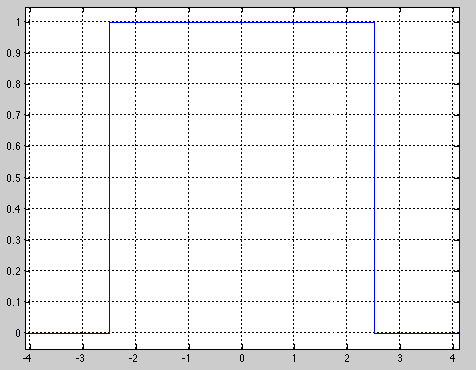
\includegraphics[scale=0.75]{images/portet.png}
    \caption{Fonction porte h(t) pout T=5}
  \end{figure}
  
  \section{Fonction porte H(f)}
  
\begin{lstlisting}

	t1 = [min:1/nbel:-2/f-1/nbel];
	t2 = [-2/f:1/nbel:2/f];
	t3 = [2/f+1/nbel:1/nbel:max];
	x=[zeros(size(t1)), ones(size(t2)), zeros(size(t3))];
	figure(1);
	plot([t1 t2 t3],x);
	grid;
	axis([min-1 max+1 -0.05 1.05]);
\end{lstlisting}
  
  \begin{figure}[h]
   \centering
    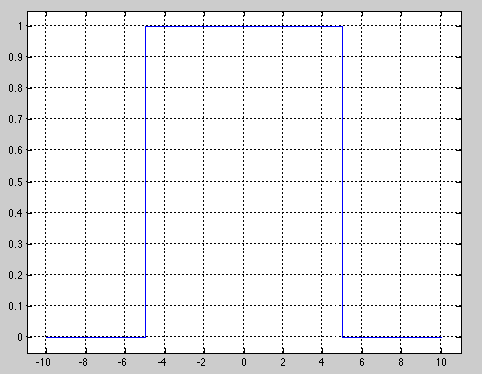
\includegraphics[scale=0.75]{images/portef.png}
    \caption{Fonction porte H(f)}
  \end{figure}
  
  \section{Interpr\'etation}
Le filtre cr\'e\'e est un filtre passe-bas id\'eal/
Ce filtre ne retient que des basses fr\'equences en att\'enuant les fr\'equence sup\'erieures \`a la fr\'equence de coupure du filtre.
La fr\'equence de coupure Fc est d\'efinie par la formule : \\
$$Fc=2*1/T=2*1/5=0,4 Hz$$
  
\newpage{}
\chapter{Application}
 	\section{Sinus cardinal}
		
\begin{lstlisting}
    t = [min:1/nbel:max];
    x = sinc(pi*1/T*t); % Signal temporel
    y = portet(T,nbel,min,max);
    x = times(x,y);
    figure(1);
    plot(t,x);
    grid;
\end{lstlisting}
		
\begin{figure}[h]
\centering
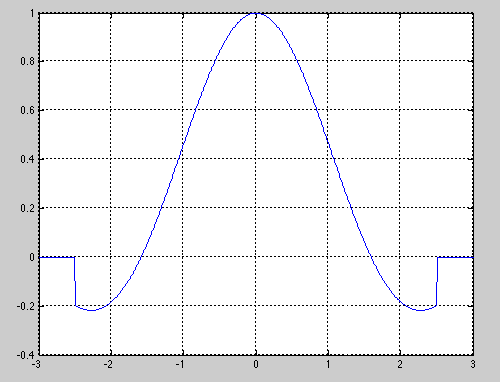
\includegraphics[scale=0.75]{images/sinc.png}
\caption{Fonction sinus cardinal}
\end{figure}

On peut voir en faisant varier la fr\'equence de coupure que plus la fr\'equence de coupure est petite, moins le filtre va conserver des fr\'equences du signal original en sortie.
En effet, le filtre passe-bas a pour caract\'eristique de ne laisser passer que les fr\'equences inf\'erieures \'a la fr\'equence de coupure. Ainsi, une fr\'equence de coupure basse restreindra d'autant la plage de fr\'equences inalt\'er\'ees.
  
 \chapter{Calcul et trac\'e de Y(f)}
 		
	\section{Application du th\'eor\`eme de Plancherel}

\begin{lstlisting}
f=20
nbel=100
max=-min=3

t=[min:1/nbel:max-1/nbel];
x=portet(1/f,nbel,min,max); %Formation d'une porte temporelle
x2 = fftshift(fft(x)); %FFT de celle ci
y=portef(f,nbel,min,max); %Formation du filtre
x2=times(x2,y); % Application du filtre 
x2=abs(x2); %Calcul de l'amplitude
figure(1);
plot(t,x2);
grid;
axis([min-1 max+1 -0.1 6.1])
end
\end{lstlisting}

		 \begin{figure}[h]
		   \centering
		    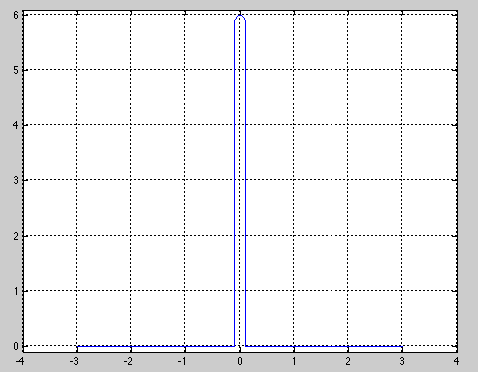
\includegraphics[scale=0.70]{images/plancherela.png}
		    \caption{Th\'eor\`eme de Plancherel}
		  \end{figure}

On voit effectivement que les fr\'equences f telles que $| f | >= 2/T$ (c'est-\`a-dire $Fc=0,4Hz$) ont bien \'et\'e supprim\'ees.
		\section{D\'emonstration du th\'eor\`eme}
		
\begin{lstlisting}
t = [2*min:1/nbel:2*max];
x = portet(1/f,nbel,min,max);
y = portef(f,nbel,min,max);
res = conv(x,y);
figure(1)
plot(t,res)
grid;
axis([min-1 max+1 -0.1 6.1]);
\end{lstlisting}
		
		 \begin{figure}[h]
		   \centering
		    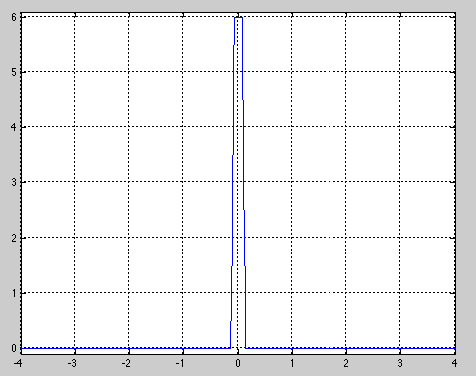
\includegraphics[scale=0.75]{images/plancherelb.png}
		    \caption{D\'emonstration graphique du th\'eor\`eme}
		  \end{figure}

Graphiquement, on voit bien ici que les deux courbes sont analogues.
On peut donc admettre le th\'eor\`eme.

\chapter{Calcul et trac\'e de Z(t)}
 
 	\section{Repr\'esentation graphique}
	
\begin{lstlisting}

t=[min:1/nbel:max];
x=plancherela(f,nbel,min,max);
x=x*f;
x=fftshift(x);
x=ifft(x);
x=abs(x);
plot(t,x)
grid
axis([min-1 max+1 -1.05 1.05])
\end{lstlisting}

	 \begin{figure}[h]
	\centering
	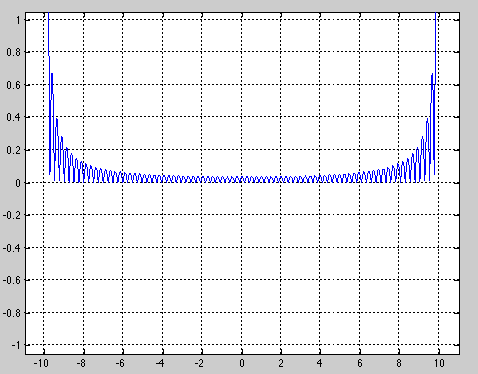
\includegraphics[scale=0.75]{images/zt5.png}
	\caption{D\'emonstration graphique du th\'eor\`eme}
	\end{figure}
En appliquant une transform\'ee de Fourier inverse, nous pouvons constater une d\'eformation du signal par rapport au signal d'origine. Ceci est d\^u \`a la perte lors du filtrage par le filtre passe bas. En effet, toutes les fr\'equences sup\'erieures \`a la fr\'equence de coupure du filtre ont \'et\'e supprim\'ees.


	\section{Z(t) pour plusieurs valeurs de fr\'equences de coupure}

Nous avons vu plus haut Z(t) pour une fr\'equence de coupure de 5Hz.
 
 	\begin{figure}[h]
	\centering
	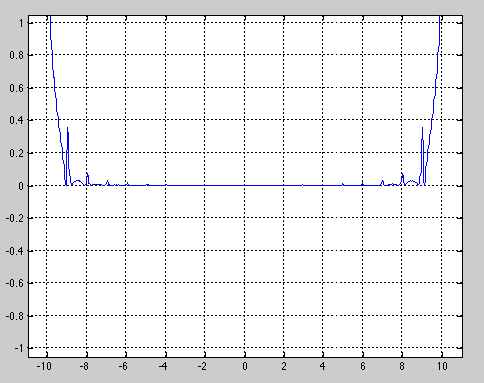
\includegraphics[scale=0.75]{images/zt1.png}
	\caption{Z(t) pour une fr\'equence de coupure de 1Hz}
	\end{figure}
	
	 \begin{figure}[h]
	\centering
	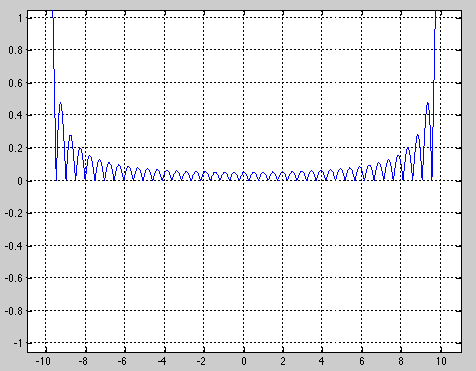
\includegraphics[scale=0.75]{images/zt10.png}
	\caption{Z(t) pour une fr\'equence de coupure de 10Hz}
	\end{figure}
	

L'augmentation de la fr\'equence de coupure nous rapproche de plus en plus de notre signal de d\'epart \`a savoir la fonction porte h(t) avec T=5.

 \chapter{Bilan}
 
 Afin qu'un signal de sortie soit identique au signal d'entr\'ee apr\`es une application d'un filtre passe-bas, il faudrait que la fr\'equence de coupure de celui ci soit sup\'erieure \`a la fr\'equence maximale du signal, donc id\'ealement que la fr\'equence de coupure soit infinie.
 \\
 Ainsi, lors d'une conversion, plus la fr\'equence de coupure du filtre est haute, plus le signal obtenu est proche de celui d'origine.
  
\end{document}